\section{遅延聴覚フィードバックが身体運動に与える影響の調査}
\subsection{調査方法}
聴覚フィードバックの遅延時間を多様に設定し,一定間隔でのボタン押下時の時間間隔のばらつきを調査した.
改良したシステムでは,ボタンの押下回数が4の倍数に達するごとに遅延を発生させた.
遅延時間は被験者には非公開として,発生させる遅延時間の順番はランダムとした.
設定した遅延時間は,実験Aでは20ms間隔で10-110ms,実験Bでは5ms間隔で10-40msとした.
実験Aの被験者は若年者(21-25歳)38名と高齢者(60-82歳)41名,実験Bの被験者は若年者(20-25歳)34名と高齢者(60-64歳)40名である.
ボタン押下の間隔は毎分80回,ボタン押下回数は34回とした.
遅延時間の提示順序は,最初に10[ms]を提示し,次に10[ms]以外の中からランダムに選択し提示する.
その後,残る遅延時間に10[ms]を加えたものをランダムに提示する.
得られた結果は,遅延時間に応じて各被験者の観測値の四分位範囲(IQR)と第一・第三四分位数を算出し,
外れ値を除外するために第一四分位数-1.5×IQR以下と第三四分位数+1.5×IQR以上の値を排除して,
4章で述べた評価方法により分析した.
\subsection{調査結果}
\begin{figure}[tbp]
  \centering
  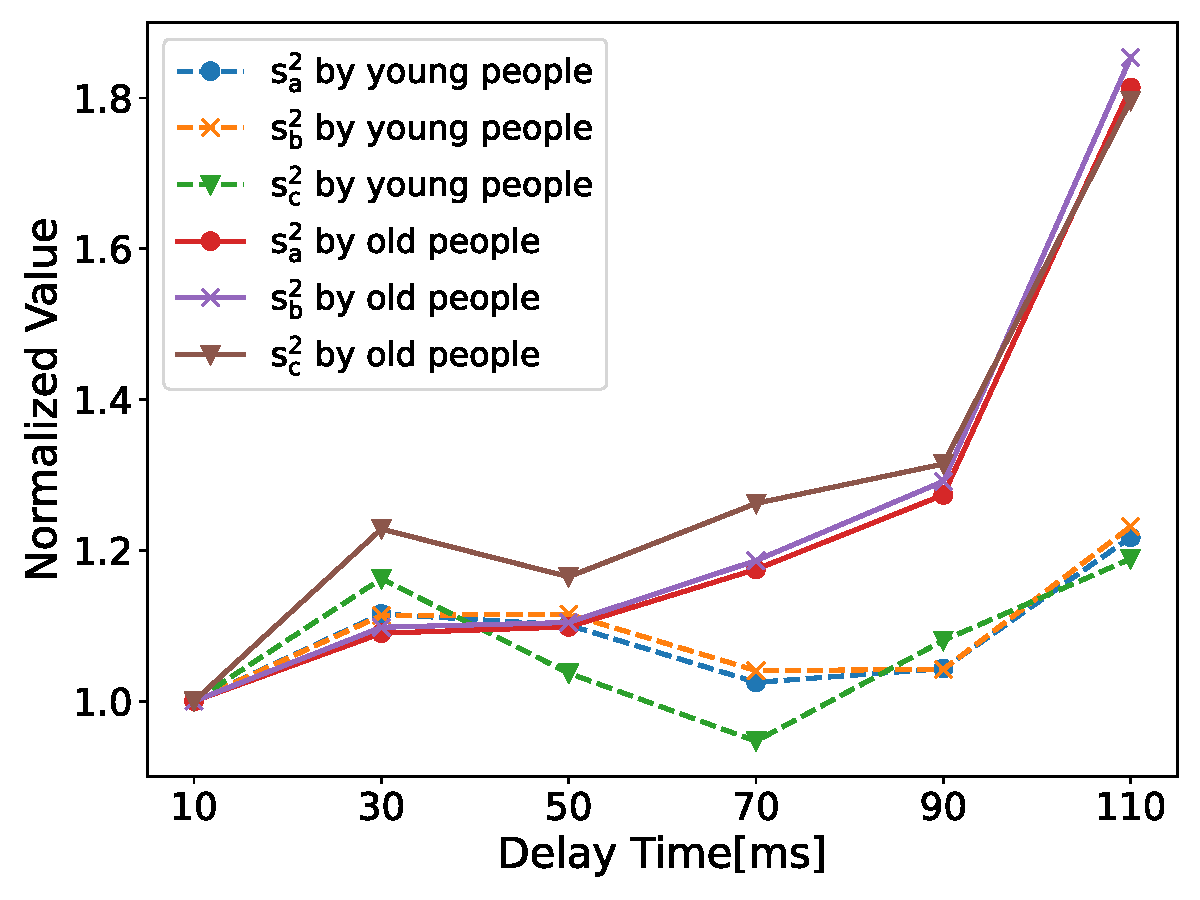
\includegraphics[scale=0.3]{figures/Honbann/Comparison_young_old/110_var_normalized.pdf}
  \caption{実験Aにおける若年者と高齢者の正規化後の評価値の比較}
  \label{fig:Normalized-Var_110ms_SaSbSc}
\end{figure}
\begin{figure}[tbp]
  \centering
  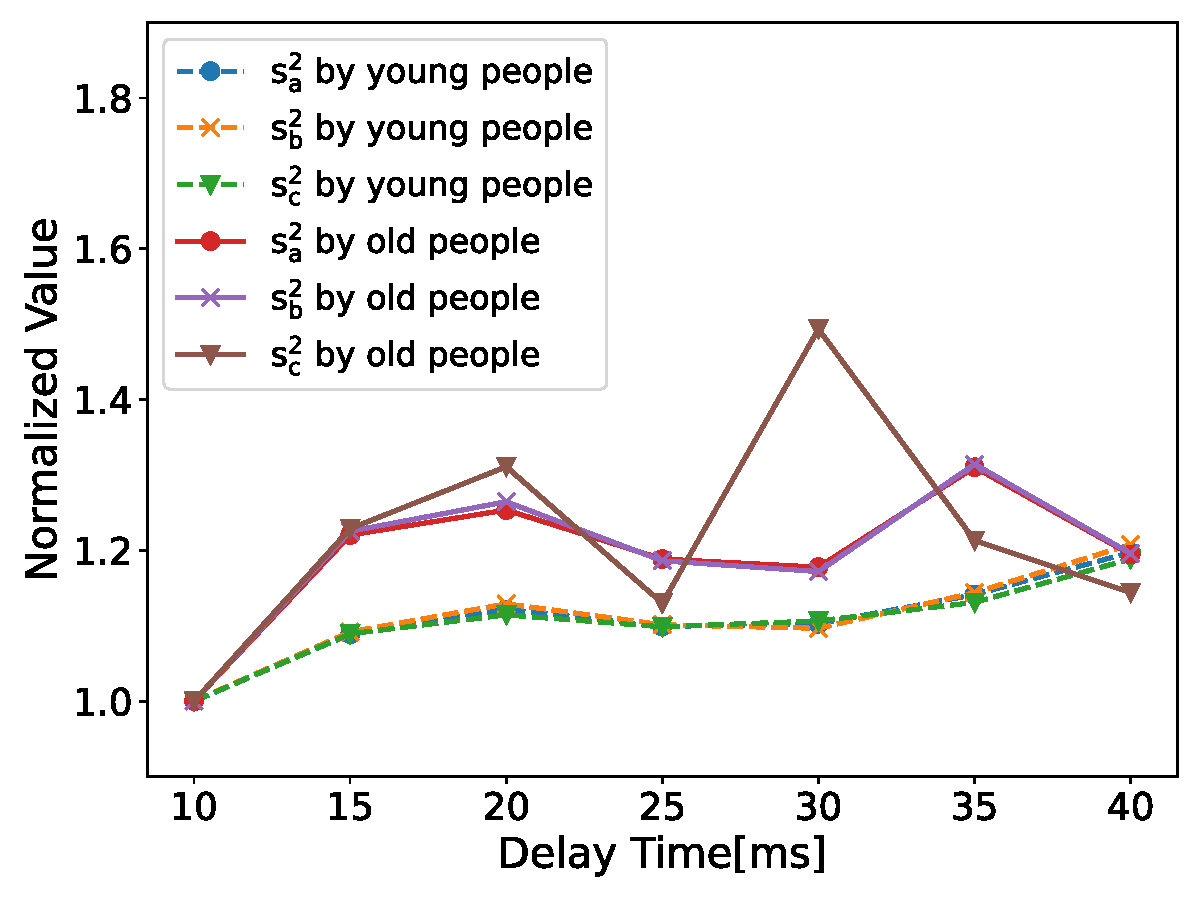
\includegraphics[scale=0.3]{figures/Honbann/Comparison_young_old/40_var_normalized.pdf}
  \caption{実験Bにおける若年者と高齢者の正規化後の評価値の比較}
  \label{fig:Normalized-Var_40ms_SaSbSc}
\end{figure}
\begin{figure}[tbp]
  \centering
  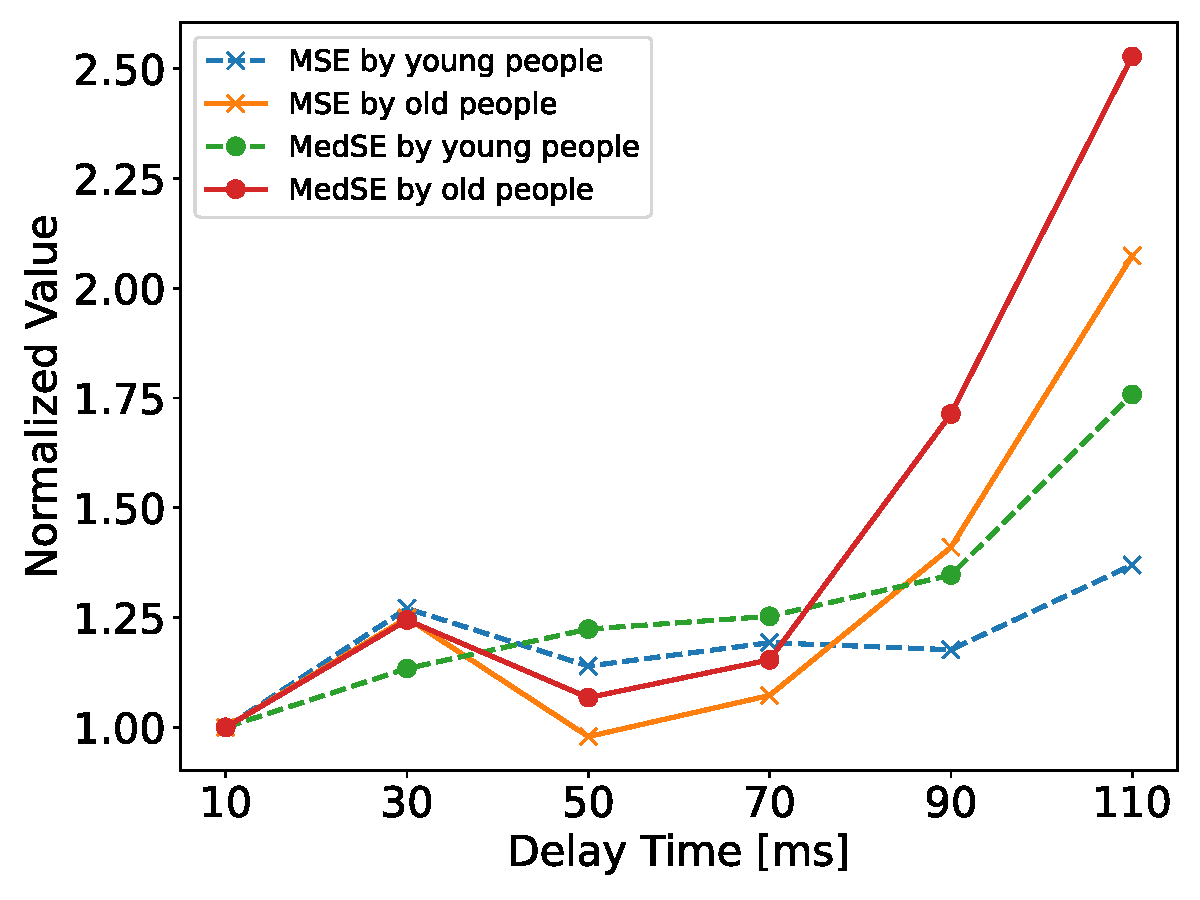
\includegraphics[scale=0.3]{figures/Honbann/Comparison_young_old/110_MSE-MedSE_normalized.pdf}
  \caption{実験Aにおける若年者と高齢者の正規化後のMSEとMedSEの比較}
  \label{fig:Normalized_110ms_MSE_MedSE}
\end{figure}
\begin{figure}[tbp]
  \centering
  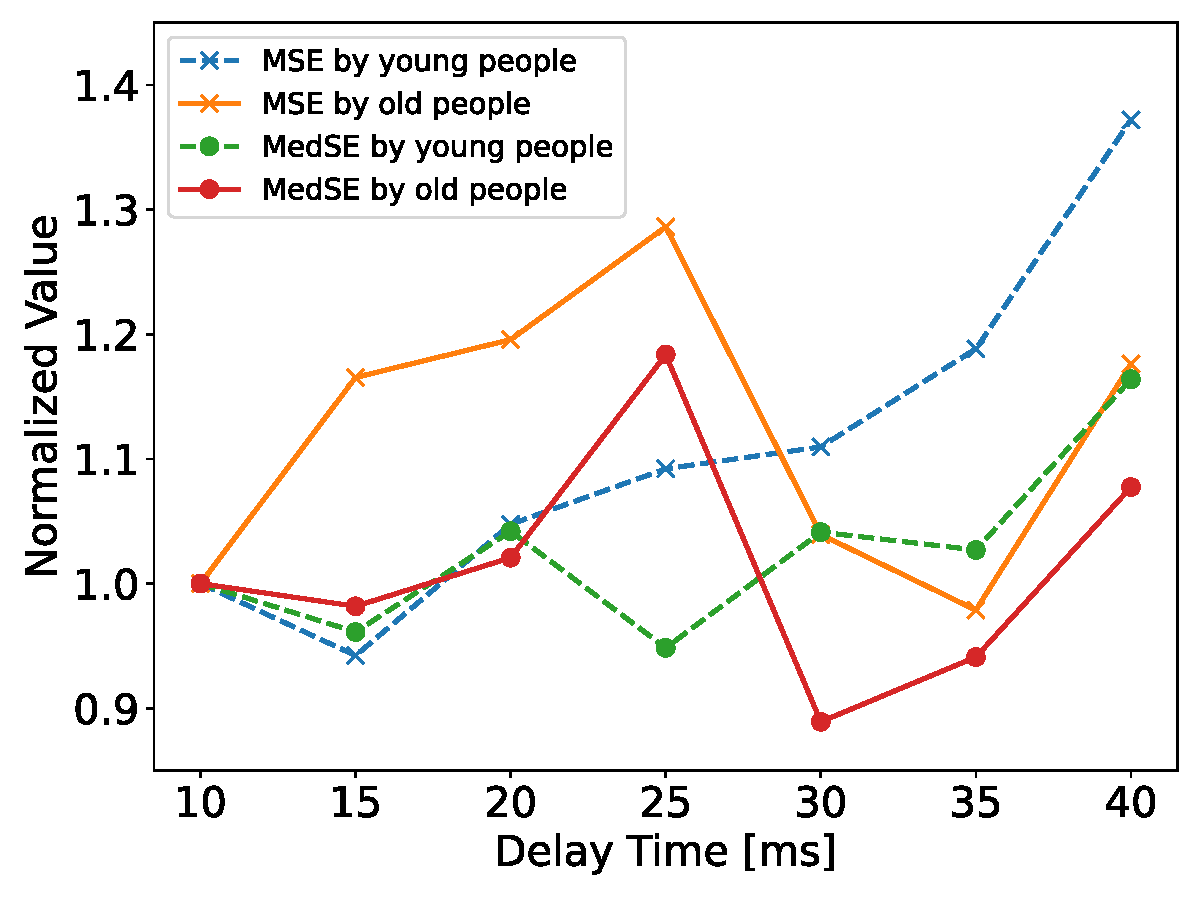
\includegraphics[scale=0.25]{figures/Honbann/Comparison_young_old/40_MSE-MedSE_normalized.pdf}
  \caption{実験Bにおける若年者と高齢者の正規化後のMSEとMedSEの比較}
  \label{fig:Normalized_40ms_MSE_MedSE}
\end{figure}